\appendix
\newpage


\section{List of Work Distribution \label{sec:ListOfWorkDistribution}}
The following list shows the estimated contribution of each member in a given part of the project. The ordering of names specifies which members have had the biggest responsibility of the component.

\begin{itemize}
	\item Architecture\\
	Split equally between all team members.
	\item Client
	\begin{itemize}
		\item Views\\
		\textbf{AWIS}, \textbf{MLIN}, \textbf{AFIN}
		\item View Models\\
		\textbf{AWIS}, \textbf{MLIN}, \textbf{ADAE}
		\item Connections\\
		\textbf{AWIS}, \textbf{MLIN}, \textbf{ADAE}
	\end{itemize}
	\item Client Tests
	\begin{itemize}
		\item View Models Tests\\
		\textbf{MLIN}, \textbf{CSJE}
		\item Connections Tests\\
		\textbf{MLIN}
	\end{itemize}
	\item Common
	\begin{itemize}
		\item DTO\\
		\textbf{AFIN}, rest of team
		\item HTTPClient toolbox\\
		\textbf{MLIN}, \textbf{AWIS}
	\end{itemize}
	\item Common Tests
	\begin{itemize}
		\item DTO\\
		\textbf{AFIN}, rest of team
		\item HTTPClient toolbox\\
		\textbf{MLIN}
	\end{itemize}
	\item Server
	\begin{itemize}
		\item Storage\\
		\textbf{AWIS}, \textbf{AFIN}, \textbf{ADAE}, \textbf{CSJE}
		\item Logic\\
		\textbf{MOALB}, \textbf{AFIN}, \textbf{ADAE}, \textbf{MLIN} 
		\item Access Control\\
		\textbf{MLIN}, \textbf{AFIN}, \textbf{AWIS}
		\item Exception Handling\\
		\textbf{MOALB}, \textbf{AFIN}
		\item History\\
		\textbf{AFIN}, \textbf{AWIS}
	\end{itemize}
	\item Server Tests
	\begin{itemize}
		\item Storage Tests\\
		\textbf{MOALB}, \textbf{AFIN}
		\item Logic Tests\\
		\textbf{AWIS}, \textbf{AFIN}, \textbf{MOALB}
		\item History Tests\\
		\textbf{AFIN}
	\end{itemize}
	\item Event
	\begin{itemize}
		\item Concurrency\\
		\textbf{ADAE}, \textbf{CSJE}, \textbf{AWIS}
		\item Access Control\\
		\textbf{AFIN}, \textbf{MLIN}
		\item Storage\\
		\textbf{AFIN}, \textbf{ADAE}, \textbf{CSJE}, \textbf{MLIN}, \textbf{AWIS}
		\item Logic\\
		\textbf{MLIN}, \textbf{MOALB}, \textbf{AFIN} 
		\item Communicators\\
		\textbf{MLIN}, \textbf{MOALB}
		\item Exception Handling\\
		\textbf{MOALB}
		\item History\\
		\textbf{AFIN}, \textbf{AWIS}
	\end{itemize}
	\item Event Tests
	\begin{itemize}
		\item Concurrency Tests\\
		\textbf{AWIS}
		\item Access Control Tests\\
		\textbf{MLIN}
		\item Storage Tests\\
		\textbf{MLIN}, \textbf{MOALB}, \textbf{AFIN}
		\item Logic Tests\\
		\textbf{MLIN}, \textbf{MOALB}, \textbf{AWIS}, \textbf{ADAE}
		\item Communicators Tests\\
		\textbf{AWIS}, \textbf{AFIN}
		\item History Tests\\
		\textbf{AFIN}
	\end{itemize}
	\item DCR graph\\
	\textbf{ADAE}, \textbf{CSJE}
	\item Workflows
	\begin{itemize}
		\item Initial draft of the Brazilian Healthcare Workflow\\
		\textbf{CSJE}, \textbf{ADAE}, \textbf{MOALB}
		\item Revised version of the Brazilian Healthcare Workflow\\
		\textbf{CSJE}, \textbf{MOALB}
	\end{itemize}
	\item SCRUM Process\\
	\textbf{CSJE}, \textbf{MOALB}
	\item Report\\
	Equally divided between all team members.
\end{itemize}

The team believes that overall the contribution has been equally divided between the members.
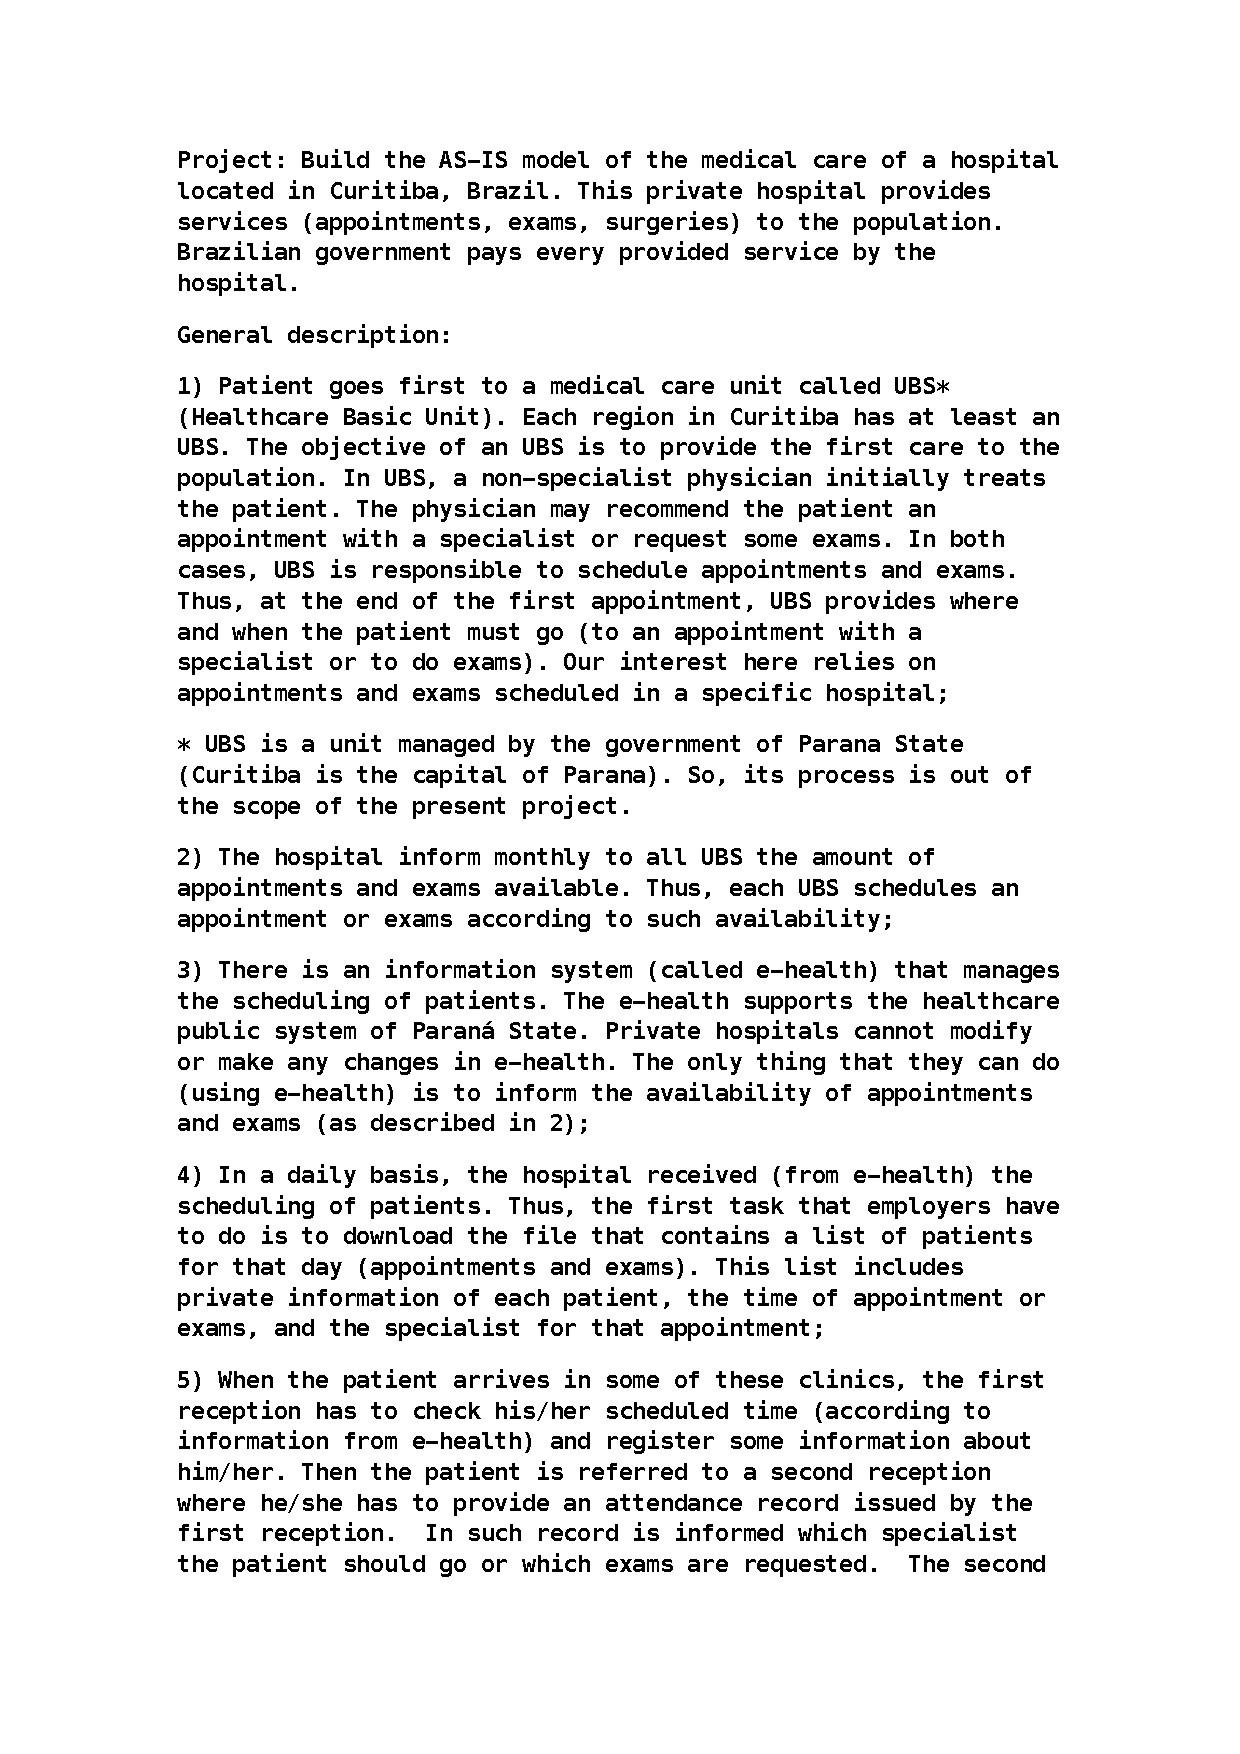
\includepdf[pages=1,scale=0.8,pagecommand=\section{Healthcare Process From Brazil}]{Figures/Appendix/HealthCareProcess.pdf}
\includepdf[pages=2-,scale=0.8]{Figures/Appendix/HealthCareProcess.pdf}

\section{Usermanual for DCR graph parser \label{sec:UsermanualForDcrGraphParser}}
The parser has only one window in which a great deal of information can be entered.\\

In the first box, called INPUT FILE, the user can write the path of a \url{DCRGraphs.net} XML-file. The user can also browse for such a file using the Choose XML-file button just below it. This will open a default Windows Open Dialog. Below the button is a box labeled Workflow Id. This is used by FlowIT to uniquely define a workflow. 

The Workflow Id should not contain spaces or symbols, but numbers, uppercase, and lowercase letters are OK.

The box labeled Workflow Name will be the name of the workflow, which the client presents. Anything can be written in this box, but if the string is too long, the Client will not be able to show everything without scrolling horizontally in the Client user interface.
In the Server Base-URL box needs to know the base URL of the server. 

This will be \url{http://flowit.azurewebsites.net/} when publishing workflows onto the hosted Azure FlowIT server. It will be \url{http://localhost:13768/} when posting to the local IIS instance when running FlowIT locally. Remember to change the Client Settings file, when running locally, see Section \ref{sec:SettingsFile} \nameref{sec:SettingsFile}).\\

The Event Base-URLs will be the base address(es) of the Event-Machines meant to host the workflow. For localhost usage it will be \url{http://localhost:13752/} (the two localhost-ports can be changed through Visual Studio or IIS-settings if desired, these are the ports the projects are configured for). 

For the hosted Azure Event Machines the addresses will be one or more of \url{http://flowites1.azurewebsites.net/}, \url{http://flowites2.azurewebsites.net/}, \url{http://flowites3.azurewebsites.net/}, or \url{http://flowites4.azurewebsites.net/}. If multiple Event Machines are desired put a comma between the base-addresses. The input is not checked before usage, so be careful what is typed into these fields.

The last textbox is the password chosen for all of the default users, which are the actors or roles from the \url{DCRGraphs.net} XML-file.

Before we get to the buttons there are two checkboxes. These are almost self-explanatory. The first one will try to create the workflow on the chosen server. This will fail if the workflow exists already. 

The second one will create the users with the typed in password, if the users does not already exist. In the case where the users are existing, the parser will not change the passwords of the existing users, it will just add the roles to the users.

The leftmost button in the bottom of the window, will parse the selected XML-file and turn it into JSON-objects which are then saved as text in graph.json which will be written to disk in the same folder as the parser-executable.

The other button will upload the parsed data directly into the Flow IT system, based on the parameters given.



\section{Possible solutions for creating the database \label{sec:SolutionsForCreatingTheDatabaseAppendix}}
In some installations it is not possible to automatically create the databases used by the Server and EventAPI. The team has identified two causes of these problems:
\begin{itemize}
\item The database instance is not created on the computer
\item The database instance has a database with the same name.
\end{itemize}


The first problem can be fixed by creating a Microsoft LocalDb instance called MSSQLLocalDb through a command line tool installed with Visual Studio.
From the Windows Command Prompt it is possible to view a list of all database instances by executing the command:\\

\indent	sqllocaldb info\\

If the list contains an entry called “MSSQLLocalDb”, this is not the cause of the problem. If “MSSQLLocalDb” is not in the list, it can be created by executing the command:\\

\indent	sqllocaldb create MSSQLLocalDb\\

Then try to restart the Server and EventAPI to see if the databases are created.\\



The second cause should not occur unless the Server or EventAPI has been run before, and the database files has been deleted. Typically the problem is that Microsoft SQL LocalDb keeps track of all of its databases and therefore it has to be removed, in order to allow the same database to be created again. The following command will tell Microsoft SQL LocalDb to stop the MSSQLLocalDb database instance:\\

\indent	sqllocaldb stop MSSQLLocalDb\\

When the instance is stopped, it can be deleted by the following command:\\

\indent	sqllocaldb delete MSSQLLocalDb\\

When this command has been executed, remember to check that the Server and EventAPI database files does not exist. These files can be found in the following directories:\\

\begin{verbatim}	   {Solution Directory}\Server\App_Data    \end{verbatim} and
\begin{verbatim}	   {Solution Directory}\Event\App_Data\end{verbatim} \\

There will be two files in each of these directories, which can safely be deleted, when the database is no longer needed.

If both the database files and the database instance is deleted, it should be possible to run the Server and EventAPI without issues. If EntityFramework cannot attach the database file, try the solution to the first cause.